  \section{Welcome: Why Git?}
  \begin{frame}[t]{Acknowledgements and Other Resources}

    \begin{itemize}
      \item Primary website: \url{http://git-scm.com}
      \item The first part of this presentation was inspired by, and copies
        from, `Git and
        Github\footnote{\url{github.com/rstudio/webinars/blob/master/2015-02/git-github.pdf}},' a webinar presented by Hadley Wickham.
      \item {\bf FREE} book: {\it Pro Git} 2nd
        edition\footnote{\url{http://git-scm.com/book/en/v2}}, best possible
        single source reference.
      \item This presentation highlights the first three chapters from
        {\it Pro Git}.
      \item A branching model I subscribe to:
        \url{http://nvie.com/posts/a-successful-git-branching-model/}

      \item Learn Git in 15 minutes: 
        \url{https://try.github.io/levels/1/challenges/1}
      \item A Simple guide and cheat sheet: 
        \url{http://rogerdudler.github.io/git-guide/}
      \item Git Videos: \url{http://git-scm.com/videos}

    \end{itemize} 
  \end{frame}

  \begin{frame}[t]
    \frametitle{Git}
    \begin{itemize}
      \item Can be difficult and frustrating to learn.
      \item Can be incorportated into your workflow.
      \item Your workflow may improve as you adapt to the git paradigm.
      \item Part of reproducable reporting.
      \item Payoffs: {\bf Safety} and {\bf Community}.
      \item Works okay for binary files 
        \begin{itemize} \item .docx, .pdf, .xlsx, \ldots \end{itemize}
      \item Works very, very, very, well for flat files: 
        \begin{itemize} \item .sas, .tex, .md, .txt, .R, .Rnw, .Rmd, .html, .c,
          .cpp, .js, .java, .csv, .dat, \ldots \end{itemize}
        
    \end{itemize}
    ``Failures, repeated failures, are finger posts on the road to achievement.
    One fails forward towards success.'' -- C.S.\ Lewis
  \end{frame}

  \begin{frame}[t]{A Story in Pictures} 
    \begin{center}
      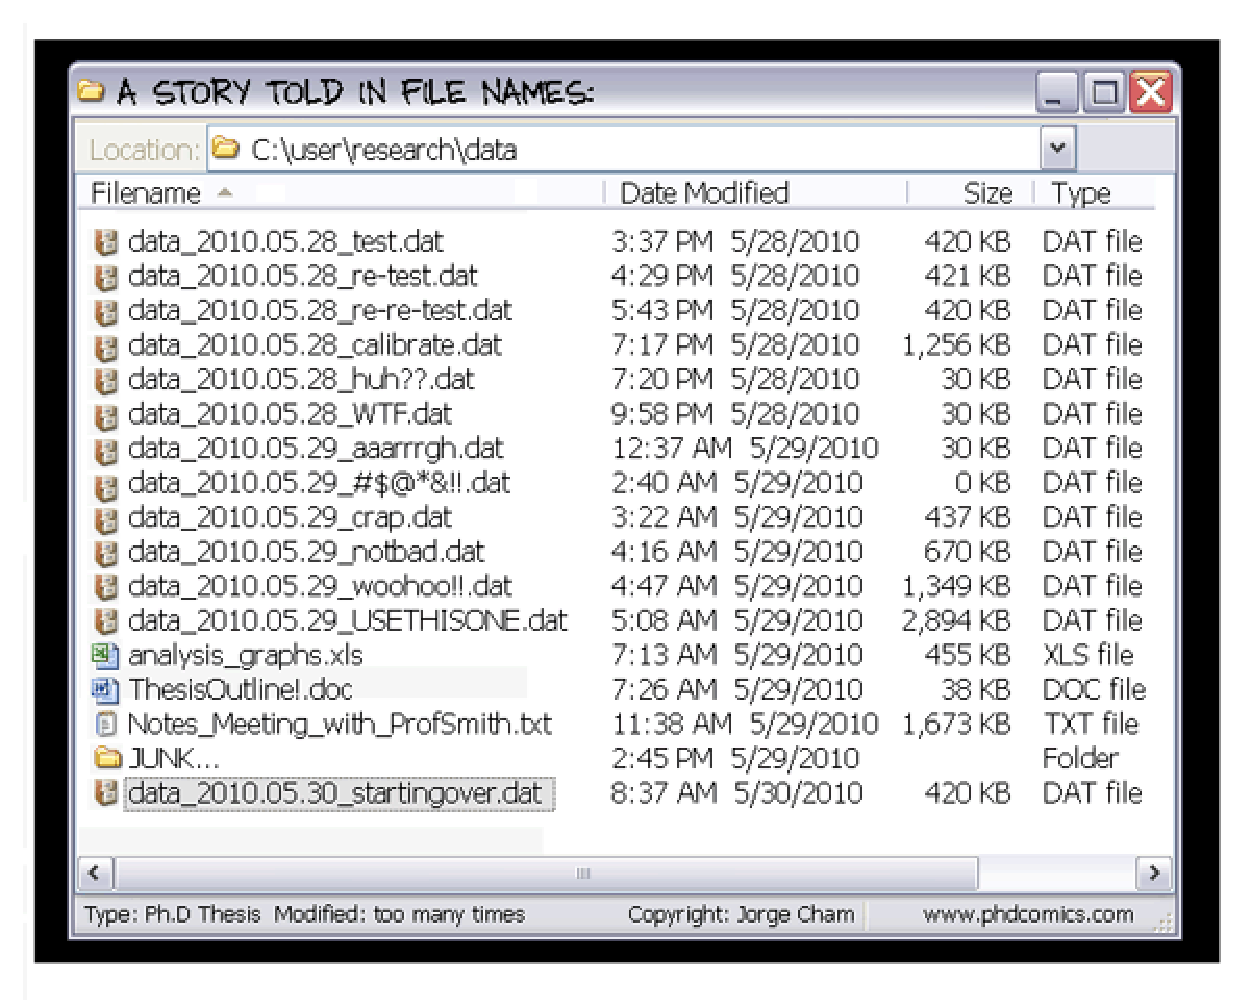
\includegraphics[height=2.350in]{../images/phd052810s} 
    \end{center} 
    \blfootnote{\url{http://www.phdcomics.com/comics/archive.php?comicid=1323}}
  \end{frame}
    

  \begin{frame}[t]{A Story in Pictures} 
    \begin{center}
      
\includegraphics[height=2.350in]{../images/phd101212s} 
    \end{center} 
    \blfootnote{\url{http://www.phdcomics.com/comics/archive.php?comicid=1531}}
  \end{frame}


  \begin{frame}[t]{A Story in Pictures} 
    \begin{center}
      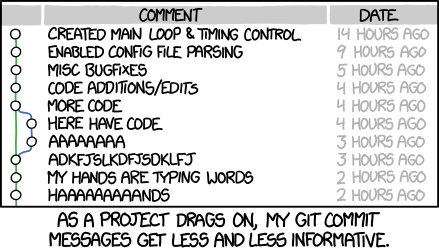
\includegraphics[height=2.000in]{../images/xkcd_git_commit} 
    \end{center} 
    \blfootnote{\url{http://xkcd.com/1296/}} 
  \end{frame}


  \begin{frame}[t]
    \frametitle{Changes}
    The history of a project can be viewed as a series of changes:
    \begin{center}
      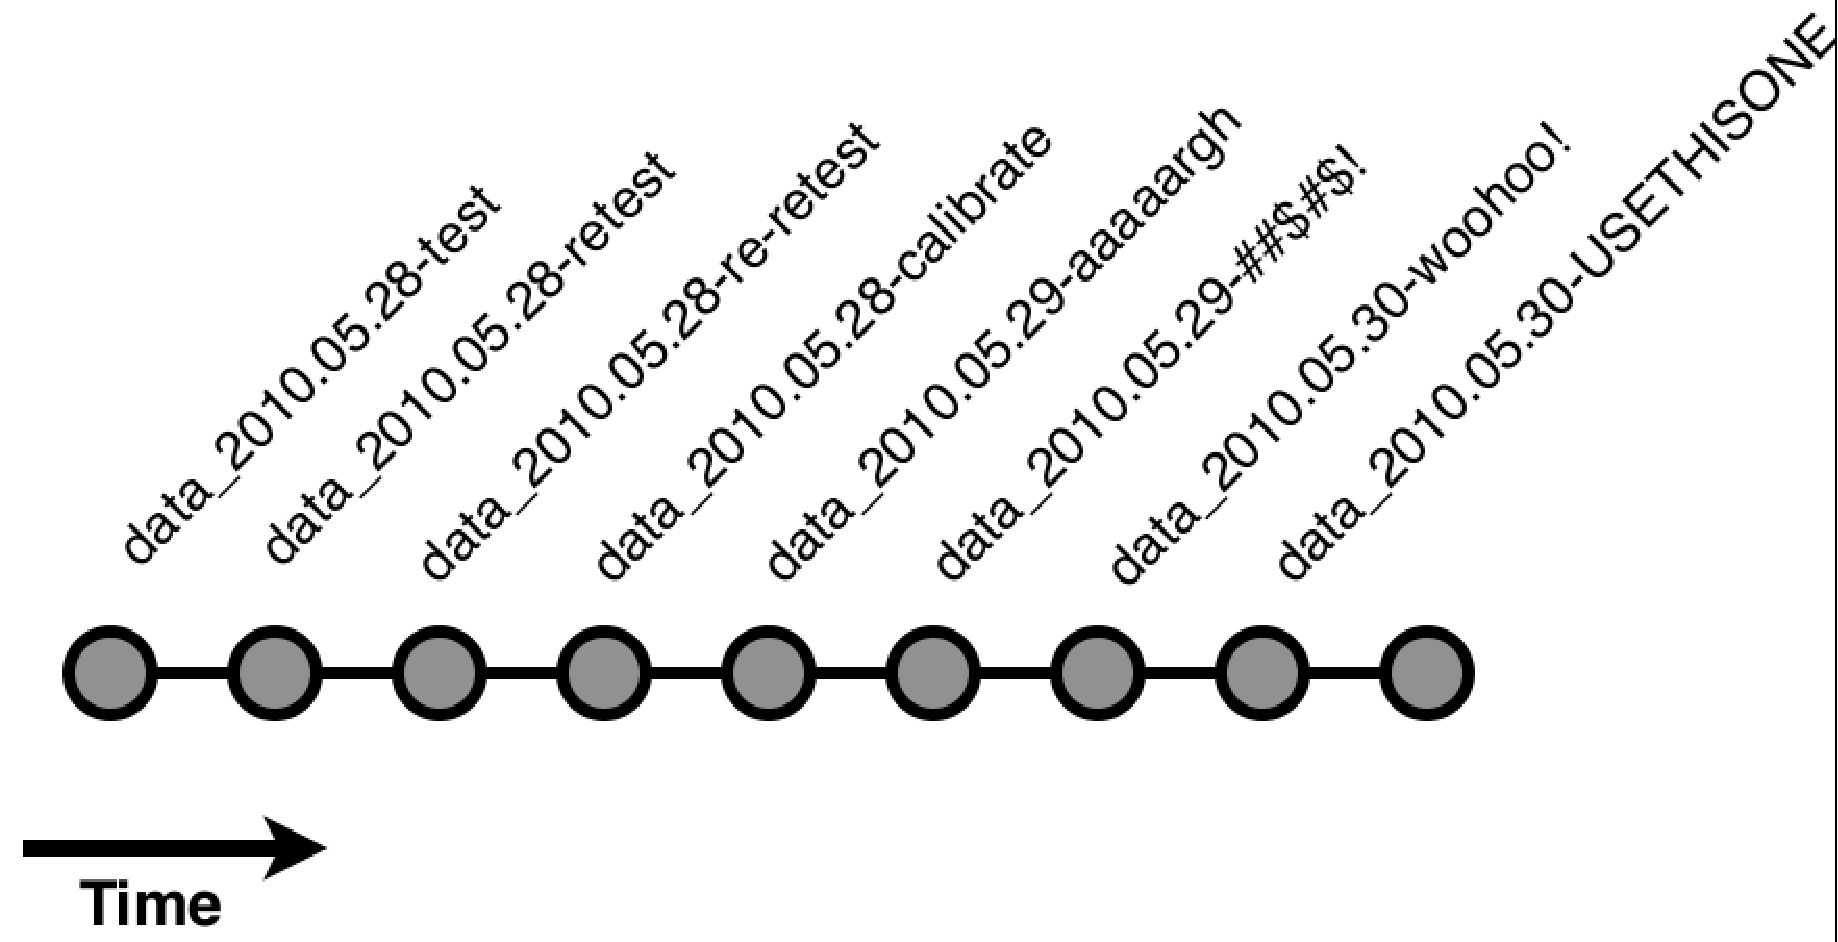
\includegraphics[height=2.00in]{../images/from-wickham-01} 
    \end{center} 
  \end{frame}

  \begin{frame}[t]
    \frametitle{Changes}
    \begin{itemize}
      \item A unique identifier
      \item What changed?
      \item When did it change?
      \item Who changed it?
      \item Why did it change?
      \item[]
      \item Difficult to coordinate with multiple files
    \end{itemize}
  \end{frame}

  \begin{frame}[t]
    \frametitle{Changes}
    With git, each change ({\bf commit}) is given a unique identifier, a {\bf
    sha}.
    \begin{center}
      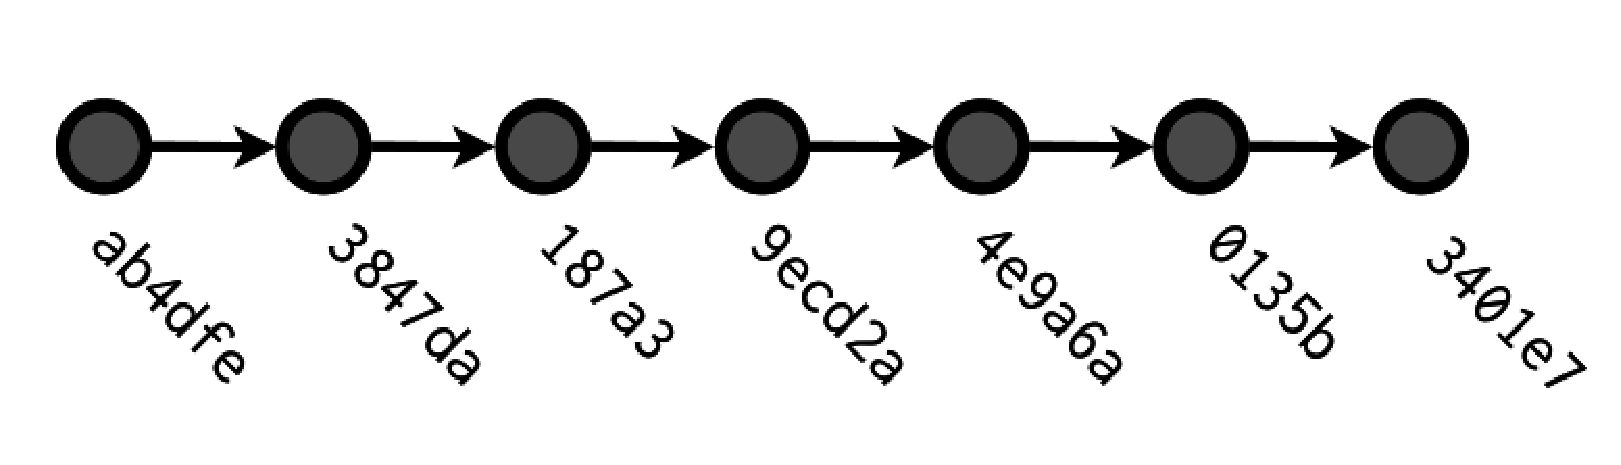
\includegraphics[width=0.98\textwidth]{../images/from-wickham-02} 
    \end{center} 

    \begin{itemize} 
      \item sha is a 40 digit long hexadecimal value.
        % $> 1.46 \times 10^{48}$ unique values
      \item sha is a key into a database that provides the author, date, and a
        description of the changes.
    \end{itemize} 
  \end{frame}

  \begin{frame}[t]
    \frametitle{Changes}
    You can also name individual commits.
    \begin{center}
      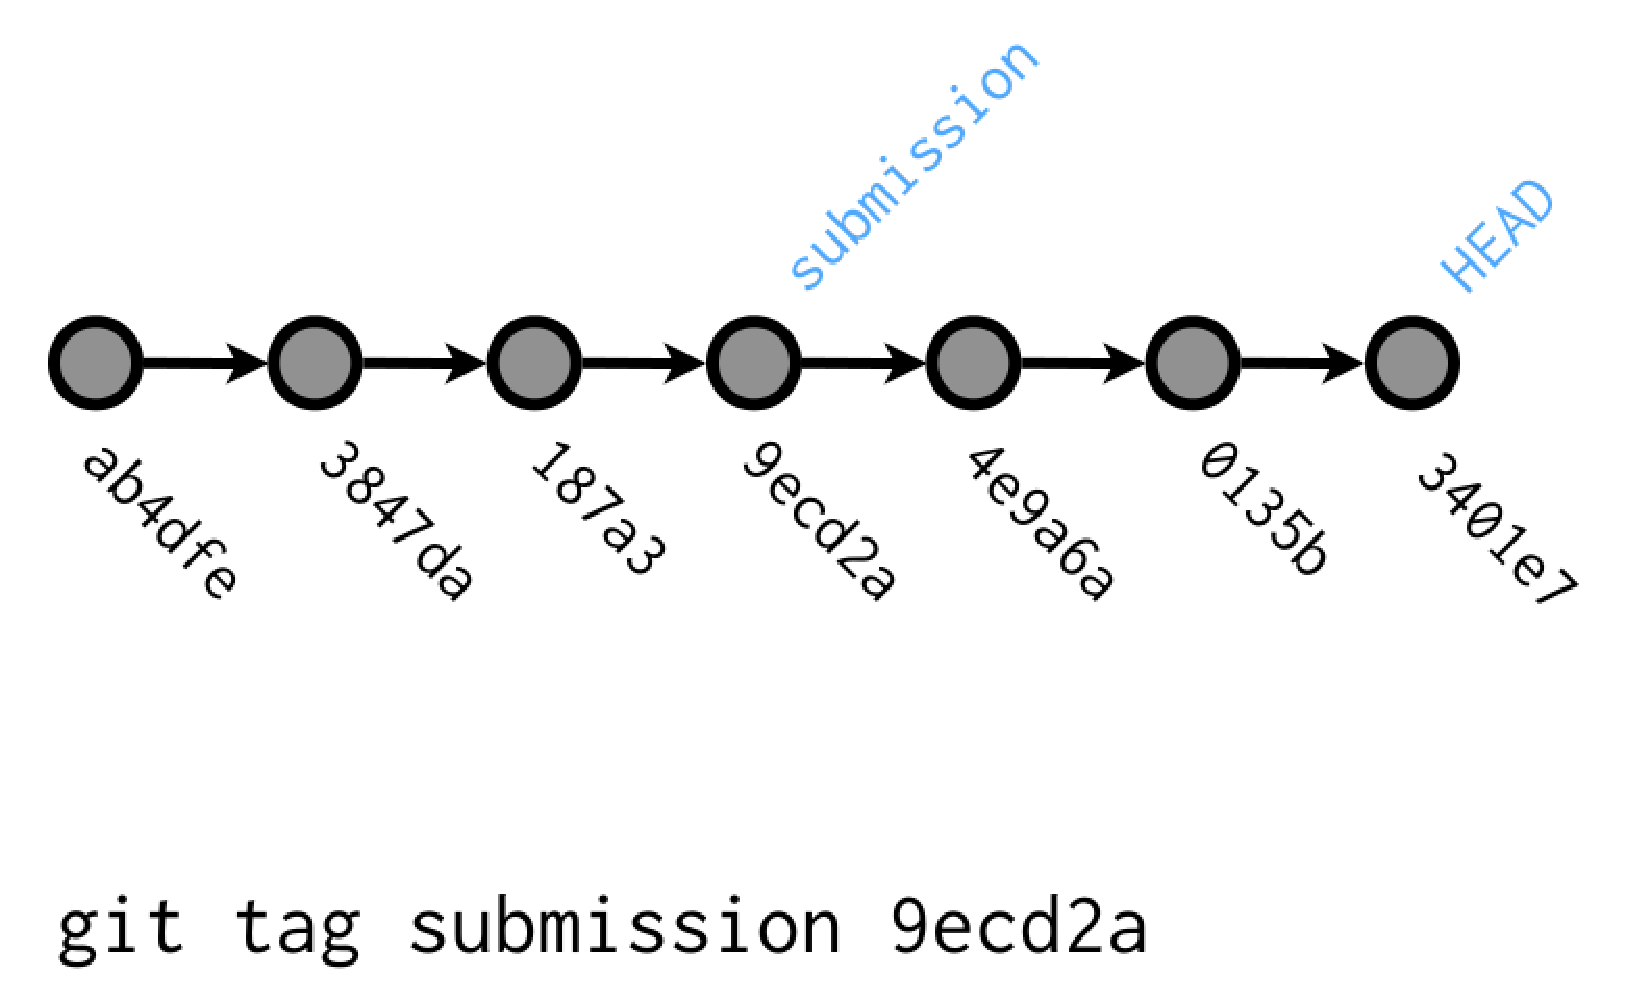
\includegraphics[height=2.00in]{../images/from-wickham-03} 
    \end{center} 

    \begin{itemize} 
      \item {\tt HEAD} is the location the working directory is set to.
      \item {\tt submission} is an example of a {\bf tag}
    \end{itemize} 
  \end{frame}

  \begin{frame}[t]
    \frametitle{Changes}
    Then see exactly what was changed 
    \begin{center}
      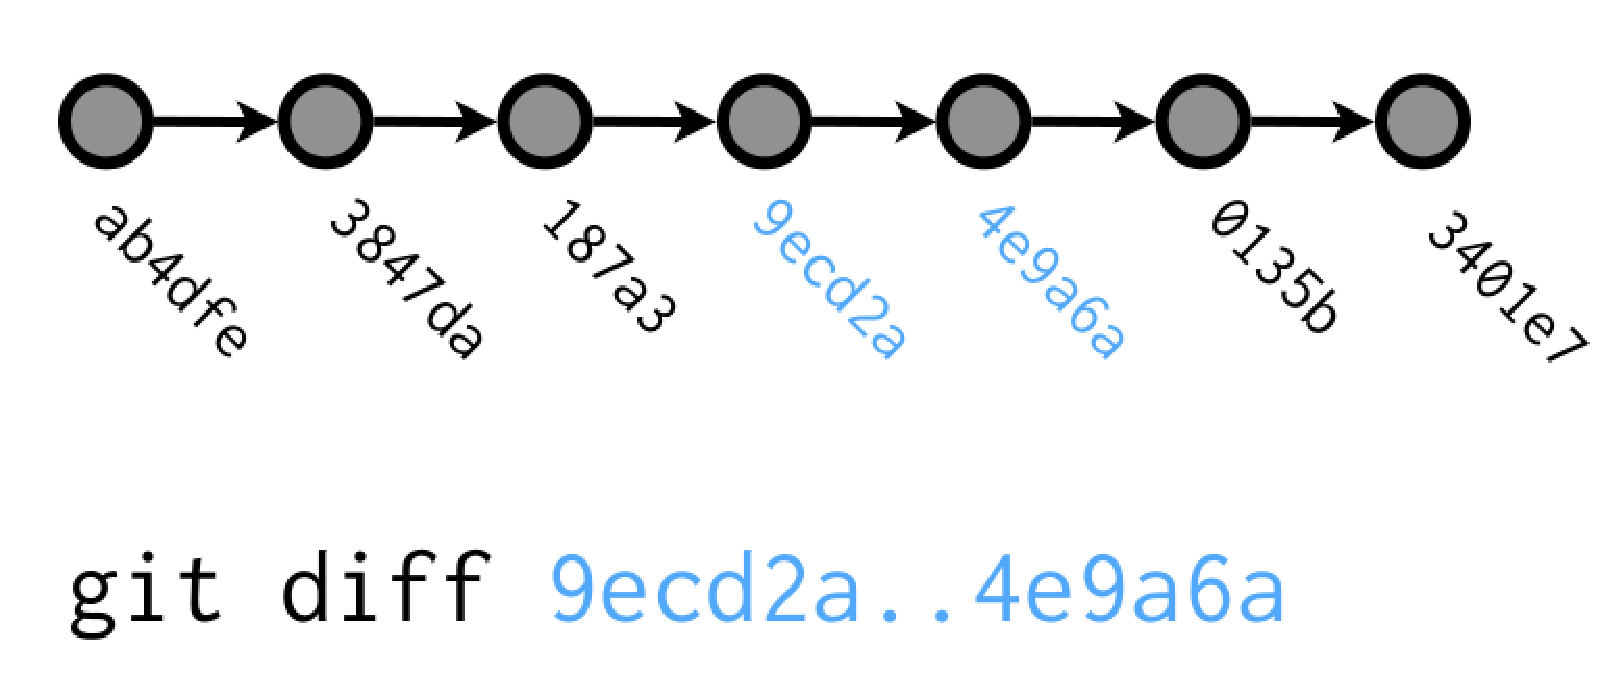
\includegraphics[height=2.00in]{../images/from-wickham-04} 
    \end{center} 
  \end{frame}

  \begin{frame}[t]
    \frametitle{Changes}
    You can revert to a previous change with git checkout
    \begin{center}
      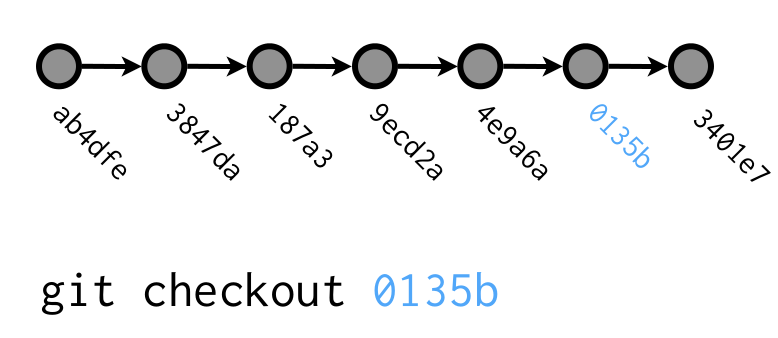
\includegraphics[height=2.00in]{../images/from-wickham-05} 
    \end{center} 
  \end{frame}

  \begin{frame}[t]
    \frametitle{Changes}
    That allows you to undo mistakes
    \begin{center}
      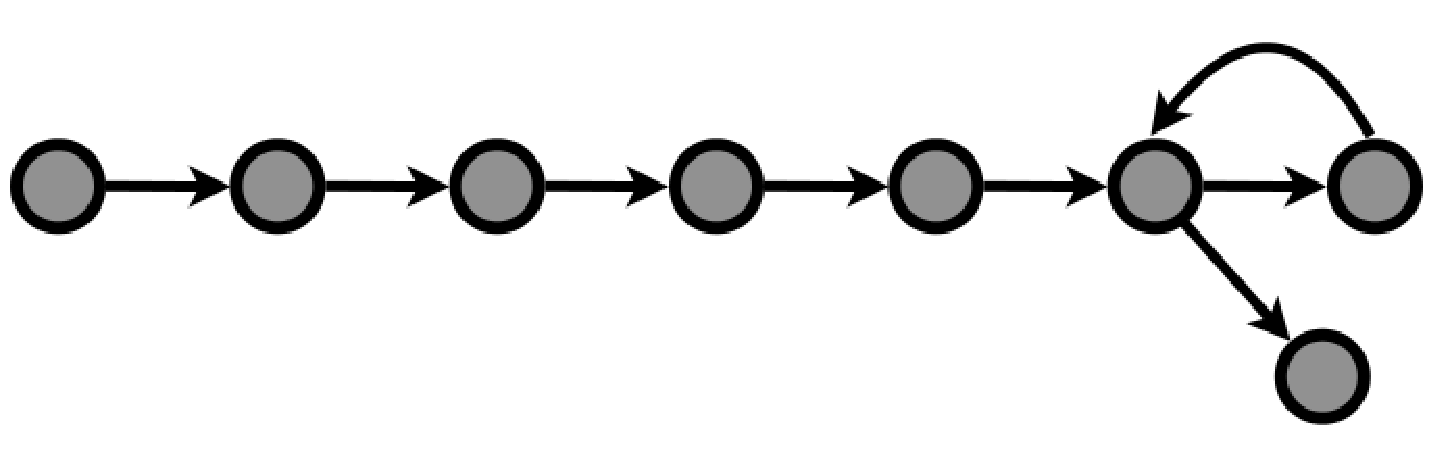
\includegraphics[width=0.98\textwidth]{../images/from-wickham-06} 
    \end{center} 
  \end{frame}
